\documentclass[10pt]{article}
\usepackage{float}
\RequirePackage{eso-pic}
\usepackage{caption}
\captionsetup[table]{labelformat=empty}



\usepackage{geometry}
\geometry{
a4paper,
left=11mm,
right=14mm,
top=37mm,
bottom=14mm,
}



\usepackage{colortbl}
\usepackage{fontspec}
\setmainfont[Ligatures=TeX]{Calibri}



\newcommand\BackgroundPic{%
\put(0,0){%
\parbox[b][\paperheight]{\paperwidth}{%
\vfill
\centering
\includegraphics{MBIE_generic_background.pdf}%
\vfill
}}}



\begin{document}
\thispagestyle{empty}
\AddToShipoutPicture{\BackgroundPic}
\section*{Key Export Statistics\footnotemark - Pet Food\footnotemark }
Published on April 07, 2016. \par
\small{\noindent{\textit{Monthly data from January 2000 to November 2015.}}}
\begin{table}[ht]
\centering
{\scriptsize
\begin{tabular}[t]{p{1.8cm}>{\hfill}p{1.4cm}>{\hfill}p{1.4cm}>{\hfill}p{1.6cm}>{\hfill}p{1.9cm}>{\hfill}p{2cm}>{\hfill}p{1.9cm}>{\hfill}p{1.5cm}}
 \textbf{Country} & \textbf{Yearly Qty} & \textbf{Yearly Value} & \textbf{Yearly Price} & \textbf{3Year CAGR(Qty)} & \textbf{3Year CAGR(Value)} & \textbf{3Year CAGR(Price)} & \textbf{Price Elasticity} \\
\hline
Australia & 13,358 & 50.5 & \$3.8 & 2.1\% & 0.2\% & -1.9\% & -1.1 \\  
China & 31,952 & 48.1 & \$1.5 & 32.1\% & 27.9\% & -3.2\% & -10.0 \\  
Indonesia & 62,337 & 43.9 & \$0.7 & -5\% & -7\% & -2\% & 2.5 \\  
USA & 12,032 & 36.0 & \$3.0 & -22.2\% & -6.5\% & 20.2\% & -1.1 \\  
Taiwan & 10,310 & 16.1 & \$1.6 & 6.1\% & 10.2\% & 3.9\% & 1.6 \\  
Japan & 4,418 & 15.1 & \$3.4 & -13.8\% & -3.1\% & 12.4\% & -1.1 \\  
Other & 34,483 & 51.3 & \$1.5 & 2.6\% & 7.1\% & 4.4\% & 0.6 \\  
Total & 168,890 & 261.0 & \$1.5 & -0.7\% & 2.5\% & 3.2\% & -0.2 \\  
\hline
\end{tabular}
}
\caption{\scriptsize Top 6 Pet Food Markets for year ending November - 2015: Quantity('000 kg) Value(NZ\$Mill), Price and their last 3-Year Growth Rates}
\end{table}


\vspace{-0.7cm}



   \begin{figure}[H]
   \centering
    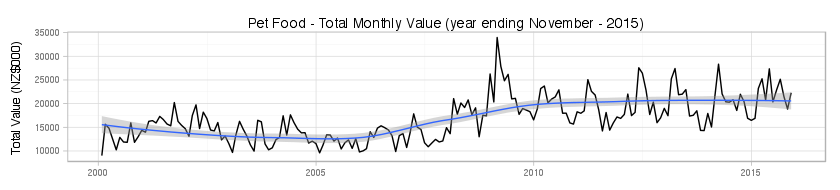
\includegraphics[scale=0.5]{../graphs/monthly_value/pet_food_monthly_value.png} \
    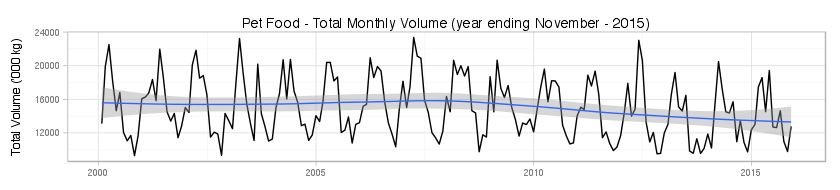
\includegraphics[scale=0.5]{../graphs/monthly_volume/pet_food_monthly_volume.png} \
    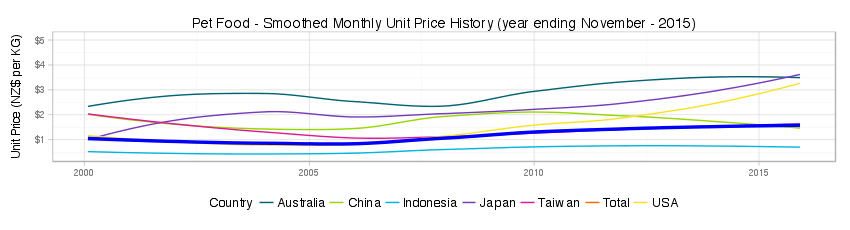
\includegraphics[scale=0.5]{../graphs/smoothed_price/pet_food_smoothed_price.png} \
    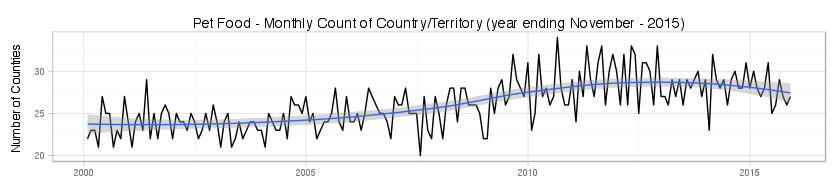
\includegraphics[scale=0.5]{../graphs/monthly_number_countries/pet_food_monthly_count.png} \
    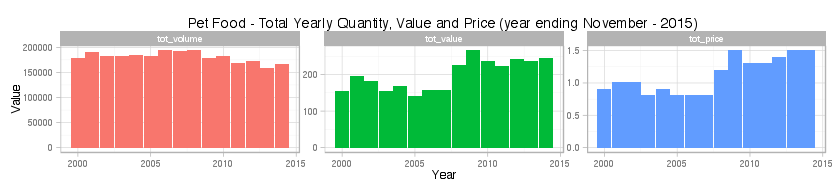
\includegraphics[scale=0.5]{../graphs/yearly_summary/pet_food_yearly_summary.png} \
   \end{figure}



\footnotetext[1]{Source: Statistics New Zealand - Overseas Merchandise Trade}
\footnotetext[2]{Harmonised System Codes for Pet Food starting with: 230110, 230120, 230910.}
\end{document}
